\chapter{绪论}
\section{xxxx}
星系形态学作为现代天文学和天体物理学的核心研究领域之一,为理解宇宙中最复杂的恒星系统~——~星系的形成与演化过程提供了重要的观测窗口\cite{Kormendy2004,Sandage2005,mo2010}。
\begin{figure}[htbp]
\centering
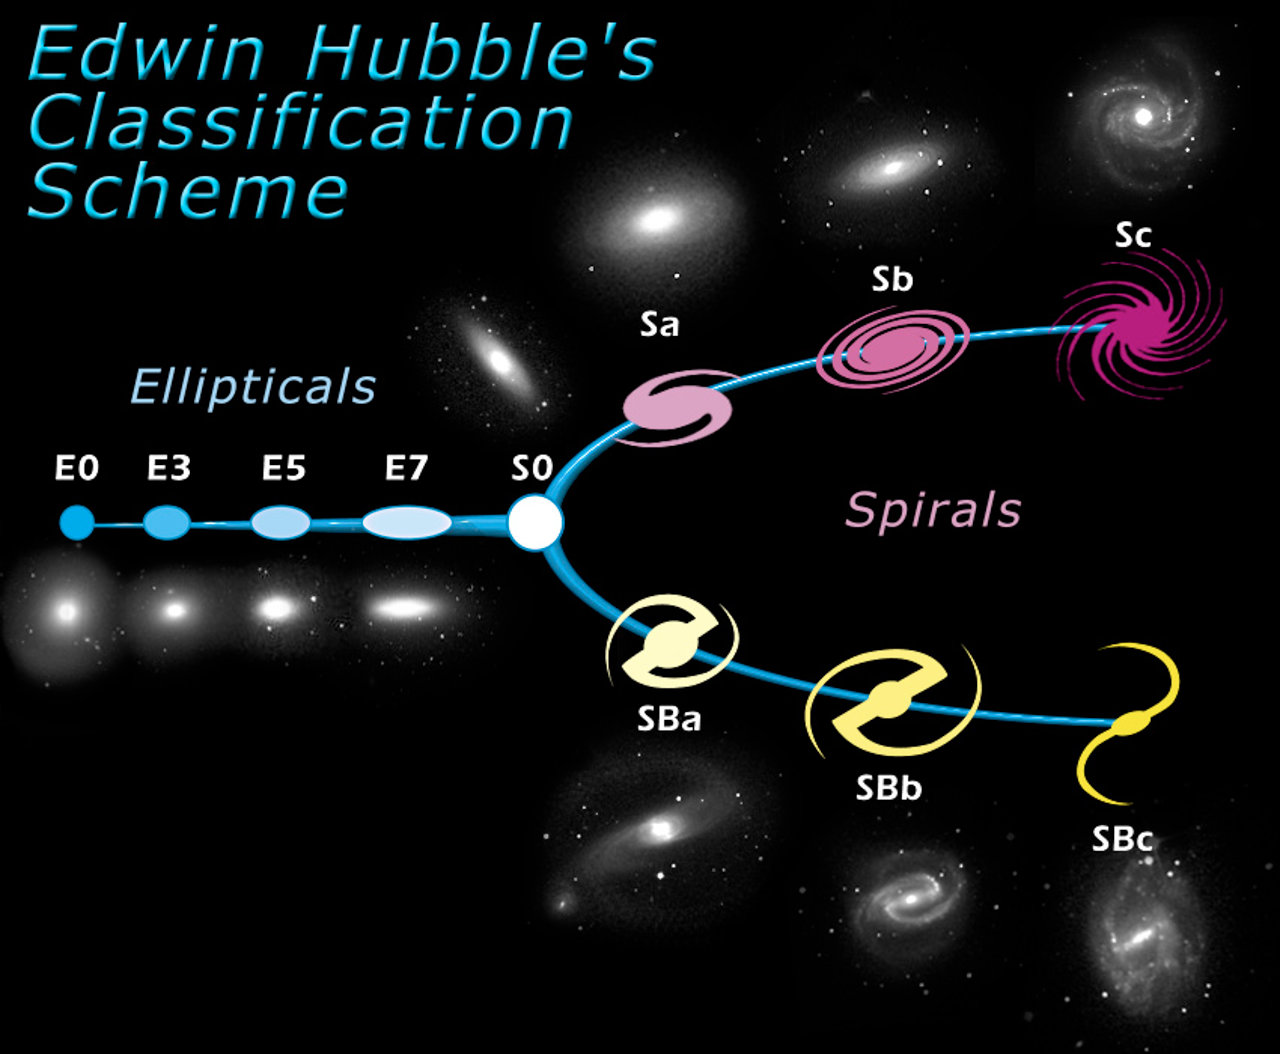
\includegraphics[width=0.45\textwidth]{Hubble_Sequence.jpg}
\caption{: \emph{Hubble Sequence示意图。图片来源:NASA\&ESA 。}}
\label{fig:hubble_sequence}
\end{figure}

表\ref{tab:simulation_parameters}:
\begin{table}[htbp]
\centering
\caption{模拟星系参数设置}
\label{tab:simulation_parameters}
\begin{tabular}{lc}
\hline
\hline
\textbf{参数} & \textbf{取值范围} \\
\hline
总星等 ($m_{\text{total}}$) & 20-28 AB mag \\
B/T比值 & 10\%-90\% \\
\hline
\hline
\end{tabular}
\end{table}

公式\ref{eq1}
\begin{equation}
I(R) = I_e \exp\left\{-k\left[\left(\frac{R}{R_{\text{eff}}}\right)^{1/n} - 1\right]\right\}
\label{eq1}
\end{equation}


\subsection{xxxxxx}

\subsection{xxxxxx}

